\documentclass{ieeeaccess}
\usepackage{cite}
\usepackage{amsmath,amssymb,amsfonts}
\usepackage{algorithmic}
\usepackage{graphicx}
\usepackage{textcomp}
\usepackage{bm}
\usepackage{booktabs}
\usepackage{multirow}
\usepackage{array}
\usepackage[hidelinks]{hyperref}

\makeatletter
\AtBeginDocument{\DeclareMathVersion{bold}
\SetSymbolFont{operators}{bold}{T1}{times}{b}{n}
\SetSymbolFont{NewLetters}{bold}{T1}{times}{b}{it}
\SetMathAlphabet{\mathrm}{bold}{T1}{times}{b}{n}
\SetMathAlphabet{\mathit}{bold}{T1}{times}{b}{it}
\SetMathAlphabet{\mathbf}{bold}{T1}{times}{b}{n}
\SetMathAlphabet{\mathtt}{bold}{OT1}{pcr}{b}{n}
\SetSymbolFont{symbols}{bold}{OMS}{cmsy}{b}{n}
\renewcommand\boldmath{\@nomath\boldmath\mathversion{bold}}}
\makeatother

\def\BibTeX{{\rm B\kern-.05em{\sc i\kern-.025em b}\kern-.08em
    T\kern-.1667em\lower.7ex\hbox{E}\kern-.125emX}}

\begin{document}

\history{Date of publication xxxx 00, 0000, date of current version xxxx 00, 0000.}
\doi{10.1109/ACCESS.2026.xxxxxxx}

\title{BMS-YOLO: A Lightweight Box-Supervised Morphology-Aware Pavement Distress Detection Model}

\author{\uppercase{Qi Liu}\authorrefmark{1}}
\address[1]{College of Big Data and Intelligent Engineering, Yangtze Normal University, Chongqing 408000, China (e-mail: 17837248232@163.com)}

\markboth
{Q. Liu: BMS-YOLO: A Lightweight Box-Supervised Morphology-Aware Pavement Distress Detection Model}
{Q. Liu: BMS-YOLO: A Lightweight Box-Supervised Morphology-Aware Pavement Distress Detection Model}

\corresp{Corresponding author: Qi Liu (e-mail: 17837248232@163.com).}

\begin{abstract}
Accurate and efficient detection of pavement distresses is essential for maintaining the safety of transportation infrastructure. Unmanned aerial vehicles (UAVs) provide an effective platform for large-scale road inspection, yet the extreme morphological diversity of distresses---from elongated cracks to compact potholes---poses a significant challenge for existing detectors. Existing YOLO-based methods struggle with high-frequency detail loss, homogeneous feature extraction, and loss functions that are misaligned with crack geometry. To address these limitations, this paper proposes BMS-YOLO (Box-supervised Morphology-aware Sparse YOLO), a lightweight detection framework that co-designs morphology-aware architecture with morphology-sensitive loss functions. Specifically, a frequency-direction detail enhancement (FDDE) module decouples feature maps into high- and low-frequency branches and applies directional convolutions to strengthen crack edges. A morphology-aware sparse mixture of experts (MorphSparseMoE) selectively activates specialized convolutional pathways via top-$k$ routing. An efficient channel attention (ECA) mechanism and a lightweight spatial pyramid pooling--cross-stage partial connection (SPPF-CSPC) structure further enlarge the receptive field while reducing parameters. At the loss level, wise intersection-over-union (WIoU) is combined with a box morphology consistency constraint that operates in log-space. A topology-guided post-processing strategy fuses fragmented crack predictions. On the UAV-PDD2023 benchmark, BMS-YOLO achieves 79.3\% mAP50 and 54.6\% mAP50:95 with only 3.8M parameters, outperforming YOLOv8n by 2.4 and 4.6 points, respectively, while maintaining 32.3 FPS on a desktop GPU. These results demonstrate that the model offers an accurate and deployable solution for UAV-based pavement inspection. With a compact footprint of 3.8M parameters and an inference speed exceeding 30~FPS, BMS-YOLO is well suited for offline batch processing of entire flight missions.
\end{abstract}

\begin{keywords}
Pavement Distress Detection, YOLOv8, Sparse Mixture of Experts, Wise-IoU, UAV Remote Sensing
\end{keywords}

\titlepgskip=-15pt
\maketitle

\section{Introduction}

\PARstart{C}{oncrete} pavements, bridges, and hydraulic structures inevitably develop various surface distresses such as cracks, potholes, and patches during long-term service due to repeated traffic loading, temperature variations, and environmental erosion. Among these distress types, cracks are the most prevalent and structurally threatening; their progressive propagation directly undermines the load-bearing capacity, waterproof integrity, and long-term durability of pavement systems. Potholes and patching areas constitute another category of region-type distresses that exhibit markedly different morphological characteristics from cracks, yet equally compromise traffic safety and structural service life. The scale of transportation infrastructure worldwide makes manual inspection impractical, creating an urgent demand for automated, high-throughput detection systems that can be deployed on unmanned aerial vehicles (UAVs) for efficient large-scale road monitoring~\cite{samadzadegan2024uavyolo, yang2025yolocompare, li2024mlyolo}.

Traditional distress detection relied on manual visual inspection complemented by image processing techniques, including edge detectors (Canny, Sobel), mathematical morphological operations, and thresholding. These methods can extract crack boundaries under idealized conditions with simple backgrounds and uniform illumination. However, they are highly sensitive to noise, shadows, and pavement texture heterogeneity, resulting in unacceptably high false-positive and miss-detection rates for practical deployment. Moreover, manual inspection is labor-intensive, subjective, and incapable of meeting the routine monitoring requirements of extensive road networks.

The advent of deep learning has fundamentally transformed automated pavement distress detection. Early approaches framed detection as an image-level classification task using VGG or ResNet, while semantic segmentation networks---notably U-Net---achieved pixel-level crack boundary delineation through encoder-decoder architectures. Segmentation methods, however, require dense pixel-level annotations, incur substantial computational cost, and produce high inference latency, rendering them unsuitable for near-real-time UAV inspection. Two-stage detectors such as Faster R-CNN improved localization accuracy through region proposal networks but suffered from prohibitive computational costs. In contrast, single-stage YOLO detectors have emerged as the dominant paradigm, achieving an exceptional balance between accuracy and efficiency. YOLOv8, in particular, introduces the C2f bottleneck structure, a fully decoupled detection head, and anchor-free prediction, representing the state of the art in lightweight object detection~\cite{kothai2024survey}. YOLO-based approaches have been increasingly applied to crack and distress detection with promising results~\cite{kothai2024survey, han2024msyolo}.

Despite these advances, directly applying standard YOLO architectures to pavement distress detection encounters fundamental limitations rooted in the unique characteristics of pavement defects. \textbf{(i)~Loss of high-frequency details.} Cracks manifest as high-frequency edge signals with sharp intensity transitions along specific orientations. Standard convolution and pooling operations, however, treat all frequency components uniformly. As a result, fine crack edges are progressively attenuated through successive downsampling. \textbf{(ii)~Extreme morphological diversity versus homogeneous feature extraction.} Cracks are elongated, line-like structures with aspect ratios frequently exceeding 10\,:\,1, whereas potholes and patches are compact, region-like structures with near-isotropic geometries. The C2f module stacks structurally identical bottleneck blocks that apply uniform convolutions indiscriminately across all spatial patterns, failing to distinguish between these morphologically distinct targets. \textbf{(iii)~Loss function misalignment.} The CIoU loss employed by YOLOv8 optimizes bounding box overlap, center distance, and aspect ratio. For elongated cracks, however, even minor positional offsets cause precipitous IoU degradation. Moreover, CIoU provides no gradient signal for non-overlapping boxes, hindering the learning of small crack fragments. \textbf{(iv)~Fragmentation.} Cracks frequently appear as discontinuous structures in aerial imagery, causing a single continuous crack to be detected as multiple overlapping boxes. Standard Non-Maximum Suppression (NMS) cannot properly consolidate such fragmented predictions.

Motivated by these challenges, we propose \textbf{BMS-YOLO} (Box-supervised Morphology-aware Sparse YOLO), a lightweight detection framework built on the core philosophy of \textit{architecture---loss co-design}: morphology-aware architectural inductive biases must be paired with complementary supervisory signals; neither alone is sufficient. Our main contributions are summarized as follows:

\begin{enumerate}
\item We design a novel \textbf{frequency-direction detail enhancement (FDDE)} module that decouples the input feature map into high- and low-frequency branches. The high-frequency branch employs directional depthwise convolutions (1$\times$5 and 5$\times$1 kernels) to selectively strengthen crack edge responses, while the low-frequency branch preserves regional context. An adaptive gating mechanism fuses the two branches, improving the model's sensitivity to subtle cracks with minimal computational overhead.

\item We propose a \textbf{morphology-aware sparse mixture of experts (MorphSparseMoE)} embedded within C2f bottleneck blocks. Four specialized experts (horizontal-line, vertical-line, isotropic, and regional) are selectively activated via a lightweight top-$k$ routing network that produces sample-level routing weights through global average pooling, enabling morphology-adaptive feature modeling with sparse expert activation.

\item We further integrate \textbf{efficient channel attention (ECA)} with a \textbf{lightweight SPPF-CSPC} structure. ECA employs 1D convolution with adaptively determined kernel size for zero-redundancy channel re-weighting, while the cross-stage partial connection design with sequential max-pooling enlarges the receptive field with negligible parameter increase.

\item We introduce a novel loss function that combines \textbf{wise intersection-over-union (WIoU)} with \textbf{box morphology consistency loss}. WIoU's center-distance-based sample reweighting assigns higher loss weights to predictions with larger center deviations, providing a hard-sample-focused gradient signal that complements the standard IoU optimization. The morphology consistency loss explicitly regularizes predicted boxes toward the elongated aspect ratios characteristic of pavement cracks in log-space, providing an explicit geometric prior that contrasts with CIoU's relative aspect ratio penalty.

\item We design a \textbf{topology-guided box fusion} post-processing strategy based on a Union-Find algorithm. Fragmented crack detections are aggregated by constructing a topological graph that encodes spatial adjacency and directional consistency, significantly reducing redundant predictions while improving detection completeness for pavement inspection applications where minimizing missed detections is operationally critical.
\end{enumerate}

Extensive experiments on the UAV-PDD2023 benchmark dataset demonstrate that BMS-YOLO achieves 79.3\% mAP50 and 54.6\% mAP50:95, outperforming YOLOv8n by 2.4 and 4.6 points respectively, while maintaining 32.3 FPS on a desktop GPU---well above the threshold for near-real-time operation in offline UAV inspection pipelines. Comprehensive ablation studies validate the effectiveness of each proposed component and confirm the co-design philosophy underlying our architecture-loss integration.

The remainder of this article is organized as follows. Section~\ref{sec:related} reviews related work in distress detection, YOLO architectures, attention mechanisms, and detection loss functions. Section~\ref{sec:method} details the proposed BMS-YOLO methodology. Section~\ref{sec:exp} presents experimental results including ablation studies, complexity analysis, and qualitative comparisons. Section~\ref{sec:concl} concludes the paper and outlines future research directions.

\section{Related Work}
\label{sec:related}

\subsection{Pavement Distress Detection Methods}

Early pavement distress detection relied on manual visual inspection complemented by automated methods derived from traditional image processing. Conventional techniques, including Canny edge detection, Sobel gradient operators, mathematical morphological operations, and global or adaptive thresholding, can extract crack boundaries under idealized conditions. However, they are highly sensitive to illumination variability, surface noise, shadowing, and pavement texture heterogeneity, resulting in unacceptably high false-positive and miss-detection rates for practical deployment~\cite{samadzadegan2024uavyolo}.

The emergence of deep convolutional neural networks has fundamentally reshaped the field. Initial approaches framed distress detection as an image-level binary classification problem, employing architectures such as AlexNet and VGG to discriminate between cracked and intact image patches~\cite{yang2025yolocompare}. While these methods automate feature extraction, they provide no spatial localization of distress instances.

Semantic segmentation networks subsequently became the dominant approach for pixel-level crack detection. U-Net and its variants achieve high-precision crack boundary delineation through symmetric encoder-decoder architectures with skip connections. The seminal DeepCrack framework~\cite{liu2019deepcrack} learned hierarchical convolutional features for end-to-end edge detection, laying the foundation for subsequent work. Frequency feature aggregation~\cite{zhu2025fdyolo} and spectrum focus transformers~\cite{wang2026highwayfreq} have been applied to weak crack segmentation. More recently, DeepCrack~\cite{wu2025tinydefect} fuses hierarchical convolutional features for end-to-end edge detection using adaptive gating. SCSNet addresses the challenge of crack segmentation under shadowed conditions by incorporating wavelet adaptive attention~\cite{chen2020gabor}. For UAV-based crack evaluation, complete inspection frameworks~\cite{qiu2023uavcrack} integrate aerial image acquisition with quantitative analysis. Despite their accuracy, segmentation models demand dense pixel-level annotations, incur substantial computational cost, and are difficult to deploy on resource-constrained edge devices.

Object detection paradigms offer a pragmatic compromise between precision and efficiency. Two-stage detectors such as Faster R-CNN~\cite{electronics2025ecayolo} have been adapted for bridge crack and tunnel lining defect detection~\cite{liu2024thermaldistress}. Single-stage detectors, particularly SSD and the YOLO family, have become the mainstream choice for real-time pavement distress detection due to their end-to-end inference and favorable accuracy-speed trade-offs~\cite{yang2025yolocompare, kothai2024survey}. Transformer-based detectors such as RT-DETR and Pavement-DETR have also been explored for multi-scale defect detection~\cite{ren2025hpsmyolo}. Semantic frequency fusion transformers~\cite{han2026semenhance} further address mixed pavement damages by integrating spectral analysis with attention mechanisms. For aerial applications, drone-optimized YOLO variants with lightweight detection heads have shown promise~\cite{farooqui2026lafyolov10}.

\subsection{Lightweight YOLO Architectures and Vision Mixture-of-Experts}

The YOLO paradigm, first introduced by Redmon \textit{et al.}~\cite{han2024msyolo}, reformulated object detection as a single regression problem, achieving unprecedented inference speed. Subsequent versions progressively enhanced performance. YOLOv2 incorporated batch normalization and anchor mechanisms. YOLOv3 introduced feature pyramids with the Darknet-53 backbone~\cite{han2024msyolo}. YOLOv4 unified a suite of regularization and augmentation techniques, including Mish activation, CSPDarknet53, SPP, and Mosaic~\cite{han2024msyolo}. YOLOv7 proposed the ELAN architecture for improved multi-scale feature propagation~\cite{xu2025sppfcspc}.

YOLOv8~\cite{kothai2024survey} represents a significant architectural evolution, replacing the C3 module with the gradient-flow-optimized C2f bottleneck, adopting a fully decoupled detection head, and transitioning to anchor-free prediction. Subsequent variants (YOLOv9t, YOLOv10n, YOLOv11n) have further refined the architecture for specific accuracy-speed regimes. Lightweight YOLO adaptations for road defect detection include wavelet-based models~\cite{wang2025moeod}, Wise-IoU-optimized crack detectors~\cite{sensors2026directional}, and attention-enhanced architectures for complex scenes~\cite{han2024msyolo}. Despite these advances, the fundamental design philosophy of stacking uniform bottleneck blocks remains unchanged, which limits adaptability to targets with heterogeneous morphological characteristics.

The Mixture-of-Experts (MoE) paradigm~\cite{oksuz2024mocae, lu2025dynamicdino} realizes conditional computation through sparse gating, activating only a subset of network parameters per input. Recently, MoE has been adapted for traffic target detection~\cite{wang2025moeod} and Fourier-domain heterogeneous defect modeling~\cite{zhang2026fouriermoee}. Originally proposed for large-scale language models, MoE has been extended to computer vision, where it enables input-dependent routing to specialized subnetworks. However, existing vision MoE methods typically design experts around capacity expansion or domain adaptation rather than target morphology. We extend this concept by designing a morphology-aware sparse expert structure with specialized branches (directional lines, isotropic, and regional patterns) tailored to the diverse geometries of pavement distresses.

\subsection{Feature Enhancement and Channel Attention Mechanisms}

Convolutional operations form the computational backbone of CNNs. Depthwise separable convolution~\cite{qu2024directional} decomposes standard convolution into per-channel depthwise filtering and pointwise projection, achieving substantial parameter reduction. Directional depthwise convolutions with anisotropic kernels (1$\times$5, 5$\times$1) have been specifically designed for oriented crack features~\cite{qu2024directional}. Dilated convolution~\cite{li2024multidirection} expands the receptive field without additional parameters by inserting gaps between kernel elements. This enables faint crack edge enhancement through dilated directional operations~\cite{li2024multidirection}. Multi-directional residual blocks~\cite{li2024multidirection} further address mixed horizontal, vertical, and oblique crack patterns by introducing learnable spatial offsets. These variants improve computational efficiency or geometric adaptability. However, they do not explicitly address the frequency-directional characteristics of crack-like targets. Recent work on frequency-domain processing~\cite{zhu2025fdyolo, plosone2026yolo11fr, wang2026highwayfreq, wang2026freqseg} has demonstrated that spectral analysis---via Fourier transform, discrete cosine transform, or wavelet decomposition---can reveal high-frequency crack edges that are attenuated by standard convolutions. Frequency feature aggregation convolution~\cite{wang2026freqseg} specifically addresses weak crack segmentation by fusing spectral components across multiple frequency bands.

In the attention domain, Squeeze-and-Excitation (SE) blocks~\cite{hu2018squeeze} model channel dependencies via global pooling and fully connected layers. ECA~\cite{wang2020eca}, by contrast, eliminates dimensionality reduction, using 1D convolution for efficient local cross-channel interaction. Adaptive kernel ECA attention~\cite{electronics2025ecayolo} has been specifically optimized for pavement multi-scale defects. Morphology-guided channel attention~\cite{asce2026morphattn} further distinguishes crack and pothole features through shape-aware re-calibration.

\subsection{Bounding Box Regression Loss Functions}

Bounding box regression loss functions have evolved from simple IoU maximization~\cite{zhang2025nwdpiu} to increasingly sophisticated formulations. Combined PIoU-NWD loss~\cite{zhang2025nwdpiu} addresses long-tail class imbalance through normalized Wasserstein distance. GIoU~\cite{rezatofighi2019giou} addresses the non-overlap problem by penalizing the area of the minimum enclosing rectangle. DIoU~\cite{zheng2020diou} incorporates center-point distance for faster convergence. CIoU further adds an aspect ratio consistency term and has become the default loss in many detection frameworks.

However, CIoU exhibits inherent limitations for crack detection. First, its IoU component degrades precipitously for elongated boxes with minor positional offsets. Second, the gradient vanishes when predicted and ground-truth boxes do not overlap, leaving small crack fragments untrained. Third, the aspect ratio term provides only relative supervision without constraining absolute scale.

Wise-IoU (WIoU)~\cite{tong2024wiou} introduces a center-distance-based sample reweighting mechanism. It assigns higher loss weights to harder samples with larger center deviations, thereby emphasizing challenging predictions during training. Recent extensions such as WIoU v3~\cite{zhou2024wiouv3} further optimize the focusing strategy with dynamic non-monotonic terms for elongated crack bounding box regression. Topological-based losses~\cite{xiao2024topoloss} have also been explored to preserve crack continuity through RGB-T fusion and geometric constraints. We adopt the base WIoU formulation and superimpose an explicit morphology consistency constraint that operates in log-space. This provides both aspect ratio and scale regularization tailored to elongated crack targets.

\section{Methodology}
\label{sec:method}

\subsection{Overall Architecture of BMS-YOLO}

The proposed BMS-YOLO enhances the YOLOv8n architecture through four structural modifications and a novel loss function. All components are designed under the co-design philosophy that morphology-aware architectural inductive biases must be paired with complementary supervisory signals. The overall architecture is illustrated in Fig.~\ref{fig:architecture}.

\begin{figure*}[!t]
\centering
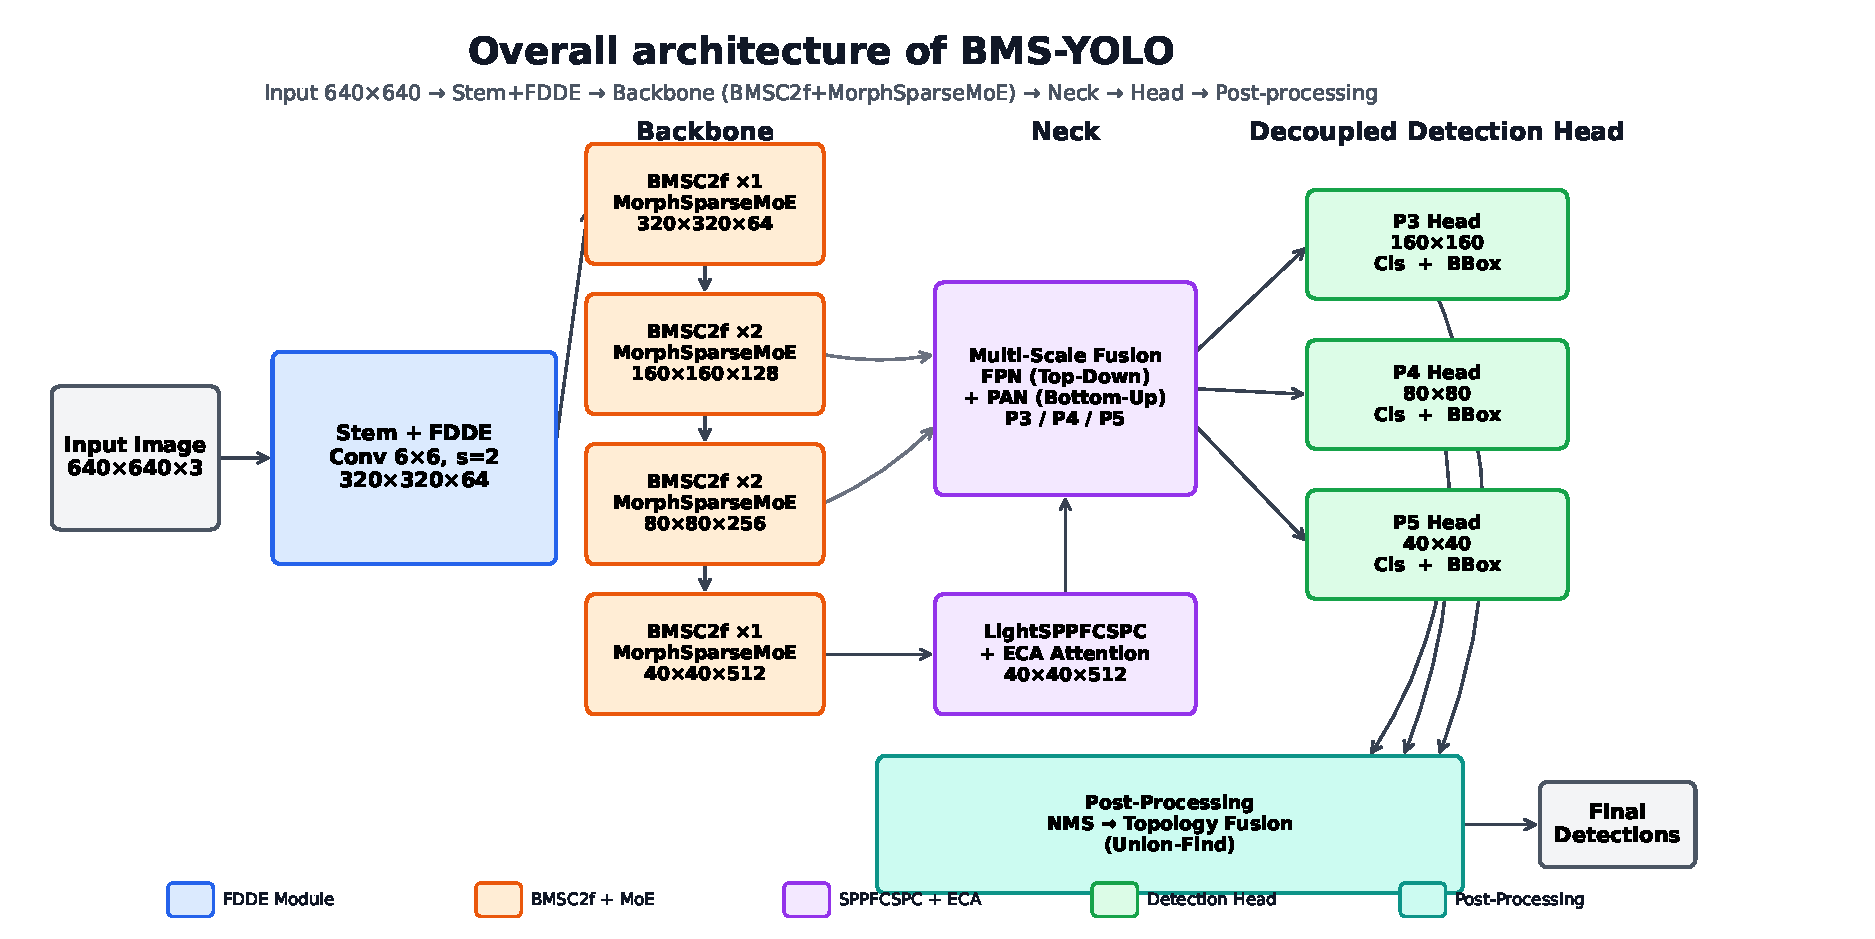
\includegraphics[width=\linewidth]{figure1_architecture.pdf}
\caption{Overall architecture of BMS-YOLO. The input image (640$\times$640) passes through a stem module augmented with FDDE, followed by a backbone comprising BMSC2f blocks with MorphSparseMoE routing. Feature pyramid aggregation is performed by SPPF-CSPC with ECA. A decoupled detection head produces class and bounding box predictions. Topology-guided box fusion consolidates fragmented crack detections at post-processing.}
\label{fig:architecture}
\end{figure*}

The input image (640$\times$640) first passes through a stem module augmented with the FDDE module, which enhances high-frequency crack edges before feature extraction. The backbone comprises a sequence of BMSC2f blocks. Each block integrates MorphSparseMoE routing that dynamically selects between four specialized expert branches according to local feature patterns. The neck employs the lightweight SPPF-CSPC structure with ECA for multi-scale feature aggregation and channel re-calibration. The detection head remains fully decoupled from the backbone, following the YOLOv8 design, with separate branches for classification and bounding box regression. Finally, at the output stage, topology-guided box fusion consolidates fragmented crack predictions. The following subsections detail each component in turn.

\subsection{Frequency-Direction Detail Enhancement (FDDE)}

Cracks in pavement imagery are intrinsically high-frequency signals characterized by sharp intensity transitions along specific orientations, whereas regional defects such as potholes and repairs exhibit low-frequency, smooth intensity variations. Standard convolution and pooling operations treat all frequency components equivalently, progressively attenuating fine crack edges through successive downsampling. The FDDE module addresses this by explicitly decoupling and differentially processing high- and low-frequency components.

Given an input feature map $X \in \mathbb{R}^{C \times H \times W}$, we obtain the low-frequency component $X_{\text{low}}$ via $3\times3$ average pooling (acting as a low-pass filter) and define the high-frequency residual as $X_{\text{high}} = X - X_{\text{low}}$. The high-frequency branch applies two depthwise convolutional layers with anisotropic kernels of sizes $1\times5$ and $5\times1$, capturing horizontal and vertical linear patterns respectively. These directional responses are summed and projected by a $1\times1$ convolution to produce $X_{\text{high}}'$. The low-frequency branch is projected by a separate $1\times1$ convolution to yield $X_{\text{low}}'$.

To adaptively balance the contributions of the two branches, a gating mechanism computes channel-wise weights from the high-frequency features:
\begin{equation}
G = \sigma\big(\text{GAP}(X_{\text{high}})\big) \in (0,1)^C,
\end{equation}
where $\text{GAP}$ denotes global average pooling that reduces the spatial dimensions $(H, W)$ to $(1, 1)$ for each channel, $\sigma$ is the sigmoid activation function that maps the pooled values to the interval $(0, 1)$, and $C$ is the number of channels. The final output is computed as:
\begin{equation}
X_{\text{out}} = X + \text{Conv}_{1\times1}\Big( \big[\, G \odot X_{\text{high}}';\; (1-G) \odot X_{\text{low}}' \,\big] \Big),
\end{equation}
where $\odot$ denotes element-wise multiplication, $[\cdot;\cdot]$ denotes channel concatenation, $X_{\text{high}}'$ and $X_{\text{low}}'$ are the projected high- and low-frequency features obtained by $1\times1$ convolutions, and $X$ is the original input feature map that provides a residual connection. The residual connection ensures that the original feature information is preserved while directionally sensitive crack details are enhanced. This design introduces only two depthwise convolutions (negligible parameter increase) while substantially improving the model's responsiveness to fine linear structures.

\subsection{Morphology-Aware Sparse Experts (MorphSparseMoE)}

The C2f module in YOLOv8 stacks multiple identical bottleneck blocks, which cannot differentially process the extreme morphological variation between crack-like and pothole-like distresses. We introduce a Morphology-aware Sparse Mixture of Experts (MorphSparseMoE) block embedded within each C2f unit. This block comprises four specialized expert branches:

\begin{itemize}
\item \textbf{Expert 0 (Horizontal Line):} Depthwise convolution with kernel $1\times5$, targeting horizontally elongated structures in image coordinates.
\item \textbf{Expert 1 (Vertical Line):} Depthwise convolution with kernel $5\times1$, targeting vertically elongated structures in image coordinates.
\item \textbf{Expert 2 (Isotropic):} Standard $3\times3$ depthwise convolution, suitable for arbitrary short crack segments or oblique patterns.
\item \textbf{Expert 3 (Region):} Average pooling followed by $1\times1$ convolution, extracting large-area context for potholes and repair patches.
\end{itemize}

A lightweight router network computes a probability distribution over the four experts. The router consists of global average pooling, a two-layer MLP with SiLU activation, and a final linear layer that produces logits for each expert:
\begin{equation}
\mathbf{w} = \text{Softmax}\big(\text{Router}(X)\big) \in \Delta^4,
\end{equation}
where $\text{Router}(X)$ denotes the routing network comprising global average pooling, a two-layer multilayer perceptron (MLP) with SiLU activation, and a final linear layer producing logit scores for each expert. The symbol $\Delta^4$ denotes the 4-simplex (the set of probability vectors over the four experts). To enforce sparsity, we retain only the top-$k$ experts (we set $k=2$) by masking the remaining weights to zero and re-normalizing the selected weights. The MoE output is:
\begin{equation}
Y = \sum_{i=0}^{3} w_i \cdot \text{Expert}_i(X),
\end{equation}
followed by a $1\times1$ projection and a residual connection. This sparse routing mechanism operates at the feature-map level: global average pooling produces a single routing weight vector per feature map, determining which morphological experts receive greater emphasis for each input sample. Note that all four expert branches are evaluated and the top-$k$ masking is applied post-hoc; the sparsity serves to re-shape the effective feature combination rather than to reduce computation.

The BMSC2f block replaces the standard C2f bottleneck in both the backbone and neck of BMS-YOLO, integrating FDDE at the input stage and MorphSparseMoE within each bottleneck iteration. The directional convolution design draws inspiration from recent work on 1$\times$5/5$\times$1 anisotropic kernels~\cite{qu2024directional} and multi-directional residual structures~\cite{li2024multidirection}. Optimized C2f variants with directional convolution~\cite{qu2024directional} have also shown improved performance for slender crack features.

% Figure 2 -- Module Structure Diagrams (FDDE / MorphSparseMoE / SPPF-CSPC)
\begin{figure*}[!t]
\centering
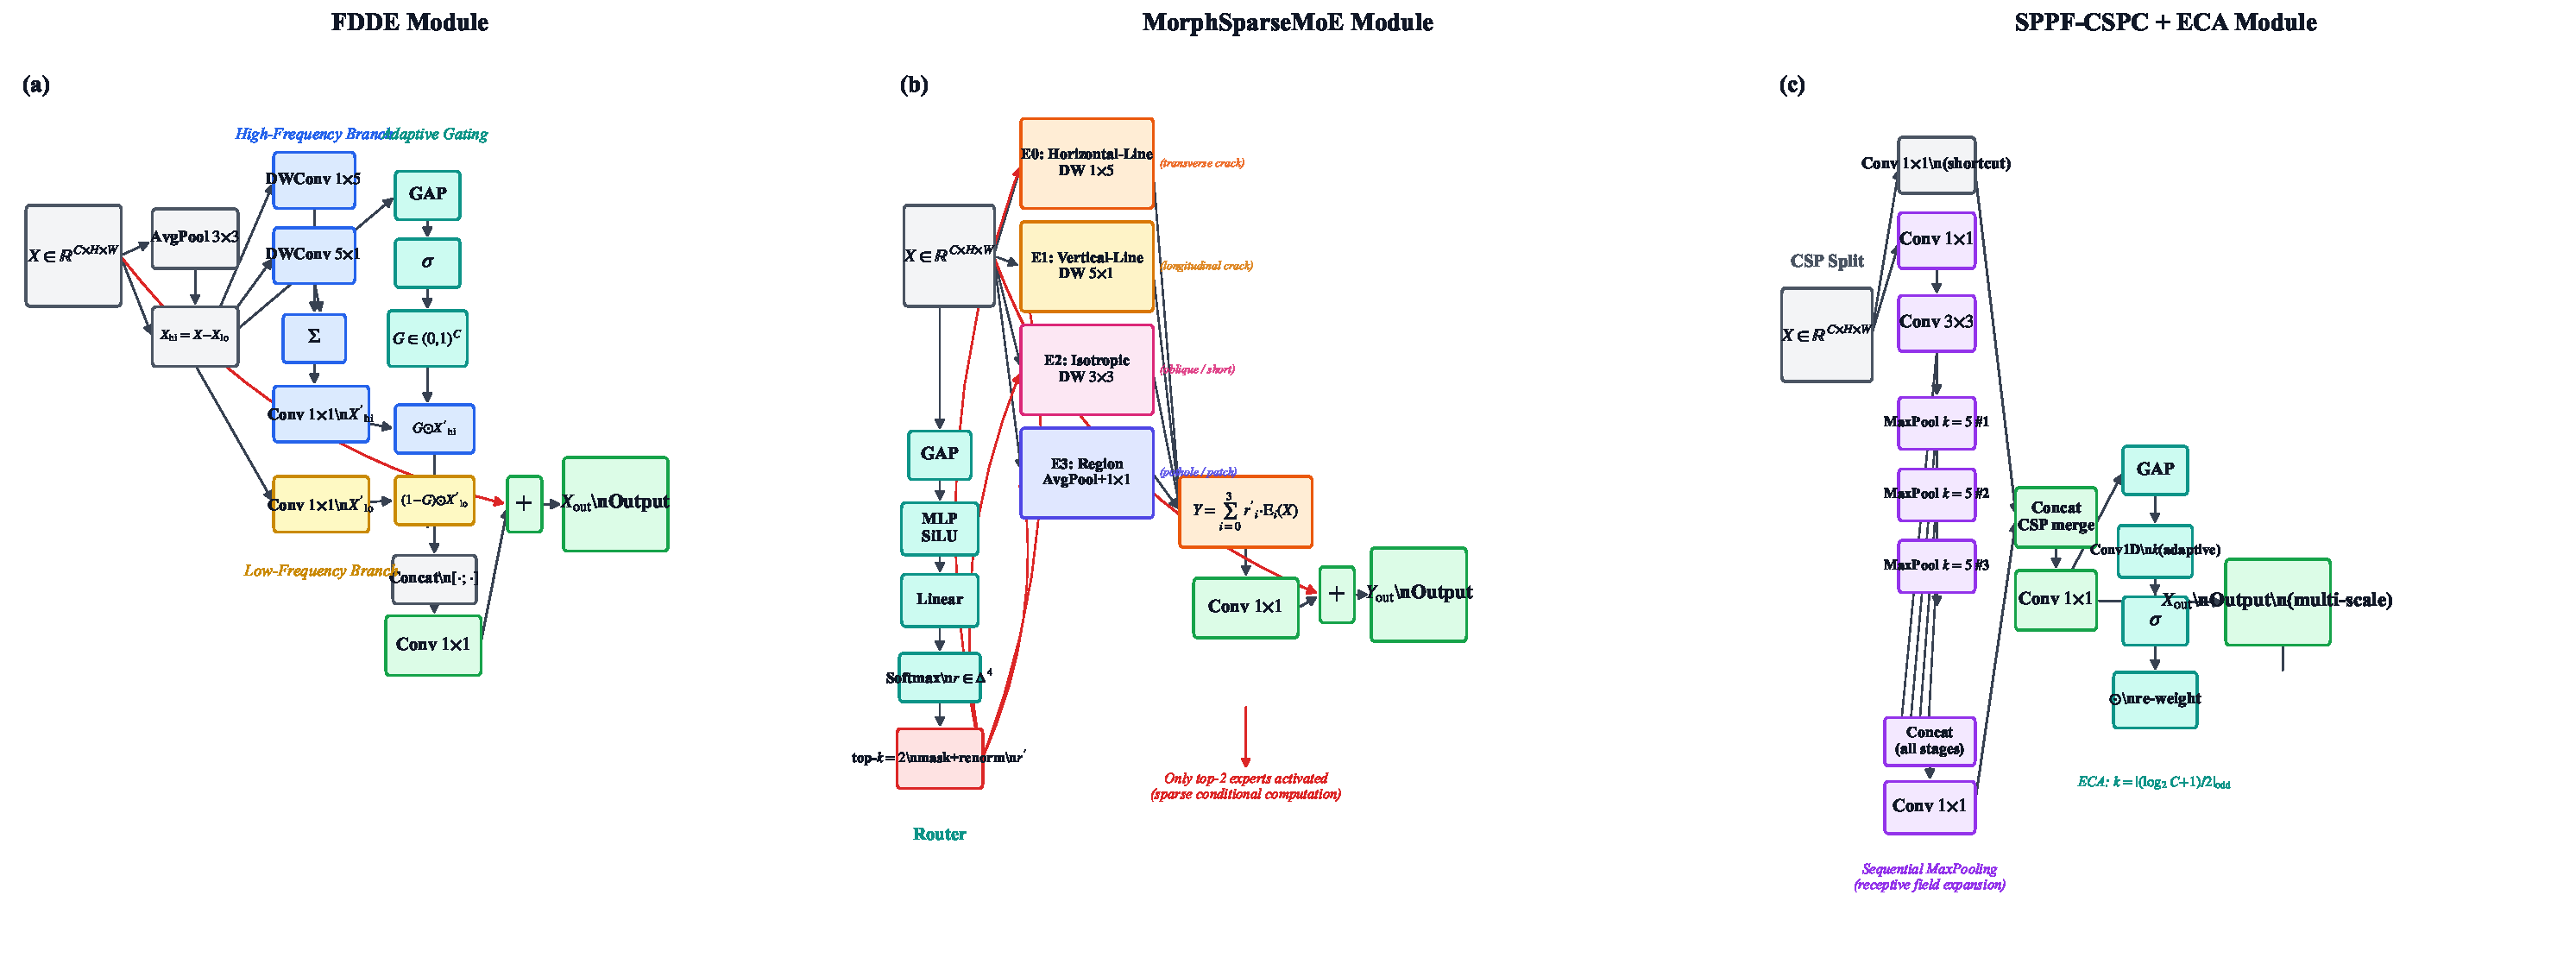
\includegraphics[width=\textwidth]{figure2_modules.pdf}
\caption{Detailed structures of the three proposed modules. (a) FDDE: the input feature is decomposed into high- and low-frequency branches; directional depth-wise convolutions ($1\times5$ and $5\times1$) enhance crack-edge responses, and a gating unit $\sigma(\text{GAP}(X_{\rm high}))$ adaptively fuses the two branches with a residual connection. (b) MorphSparseMoE: a lightweight router produces a sparse (top-$k{=}2$) distribution over four morphology-aware experts, whose weighted outputs are projected and added back through a residual connection. (c) SPPF-CSPC: a cross-stage partial split followed by sequential max-pooling ($k{=}5$) expands the receptive field at low cost, and an ECA module re-weights channels via adaptive 1D convolution.}
\label{fig:module_structure}
\end{figure*}

\subsection{Lightweight Multi-scale Fusion: SPPF-CSPC and ECA Attention}

We replace the standard SPPF module in YOLOv8 with a lightweight SPPF-CSPC variant that adopts a cross-stage partial connection (CSP) design. The SPPF-CSPC structure with cross-stage partial pooling~\cite{xu2025sppfcspc} has been shown to enhance multi-scale feature aggregation for road distress detection. The input feature is split into two branches. The first branch undergoes a $1\times1$ convolution followed by a $3\times3$ convolution, and then $n$ ($n=3$) repeated max-pooling operations with kernel size 5. Outputs from all pooling stages are concatenated and projected by a $1\times1$ convolution. The second branch is a shortcut $1\times1$ convolution. The two branches are concatenated and passed through a final $1\times1$ convolution. This design enlarges the receptive field with minimal parameter increase, since pooling operations are parameter-free. It enhances multi-scale feature aggregation, which is particularly beneficial for detecting both thin, elongated cracks and large potholes within the same aerial image.

At the output of both the modified C2f blocks and the SPPF-CSPC structure, we incorporate the Efficient Channel Attention (ECA) module to refine channel-wise feature representation. Unlike the Squeeze-and-Excitation (SE) block that employs dimensionality-reduction fully connected layers, ECA directly learns channel weights via 1D convolution with an adaptively determined kernel size.

Given an input feature map $X \in \mathbb{R}^{C \times H \times W}$, global average pooling yields a channel descriptor $\mathbf{z} \in \mathbb{R}^C$. The kernel size $k$ is computed as:
\begin{equation}
k = \left| \frac{\log_2(C) + 1}{2} \right|_{\text{odd}},
\end{equation}
where $C$ denotes the number of input channels and $|\cdot|_{\text{odd}}$ rounds to the nearest odd integer. The scope of local cross-channel interaction thus scales with the channel dimension. The channel weights are then $\sigma(\text{Conv1D}_{k}(\mathbf{z}))$, applied element-wise to the original feature map, where $\sigma$ is the sigmoid activation function. ECA introduces negligible computational overhead while consistently improving the model's discriminative power across all distress categories.

\subsection{Joint Loss: WIoU and Box Morphology Consistency with Two-stage Training}

YOLOv8 employs CIoU loss for bounding box regression. While effective for generic objects, CIoU exhibits limitations for pavement crack detection. First, the IoU component degrades rapidly for elongated boxes with minor positional deviations. Second, zero gradients are produced for non-overlapping boxes, impeding the learning of small crack fragments. Third, the aspect ratio term provides only relative supervision without constraining absolute scale.

We replace CIoU with Wise-IoU (WIoU)~\cite{tong2024wiou, zhou2024wiouv3}, which introduces a center-distance-based sample reweighting:
\begin{equation}
\mathcal{L}_{\text{WIoU}} = (1 - \text{IoU}) \cdot \exp\left( \frac{\rho^2}{\sigma^2} \right),
\end{equation}
where $\text{IoU}$ is the intersection-over-union between the predicted and ground-truth bounding boxes, $\rho$ is the Euclidean distance between the center points of the two boxes, and $\sigma$ is the diagonal length of the minimum enclosing rectangle covering both boxes. The exponential term is detached from the gradient to serve as a sample-dependent weighting factor, which emphasizes harder samples (those with larger center deviations) during training without altering the gradient direction of the underlying IoU loss.

Furthermore, we introduce an auxiliary morphology consistency loss that explicitly supervises the shape characteristics of elongated defects. Operating in log-space to balance the contributions of large and small boxes:
\begin{equation}
\mathcal{L}_{\text{morph}} = \delta\!\left( \log\frac{w_p}{h_p} - \log\frac{w_t}{h_t} \right) + 0.5 \cdot \delta\!\left( \log\sqrt{w_p h_p} - \log\sqrt{w_t h_t} \right),
\end{equation}
where $w_p$ and $h_p$ denote the width and height of the predicted bounding box, and $w_t$ and $h_t$ denote the width and height of the ground-truth bounding box. The function $\delta(x) = x^2/2$ for $|x| < 1$ and $\delta(x) = |x| - 0.5$ otherwise (smooth L1 / Huber loss). This provides gradient stability for large deviations while preserving the $\ell_1$ property near zero. The first term enforces aspect ratio consistency, directly addressing the elongated geometry of cracks. The second term regularizes the geometric mean of box dimensions to constrain absolute scale. The total box loss is:
\begin{equation}
\mathcal{L}_{\text{box}} = \mathcal{L}_{\text{WIoU}} + \lambda \cdot \mathcal{L}_{\text{morph}},
\end{equation}
where $\lambda$ is a hyperparameter that balances the contribution of the morphology consistency loss. Our experiments identify a two-stage ``strong-to-weak'' schedule ($\lambda = 0.02$ for the pre-training phase, then $\lambda = 0.005$ for the fine-tuning phase) as the optimal strategy.

\subsection{Inference Post-processing: Topology-Guided Box Fusion}

Crack instances in UAV imagery often manifest as elongated, discontinuous structures that standard Non-Maximum Suppression (NMS) fragments into multiple detections. We propose a topology-guided box fusion strategy that treats crack fragments as topologically connected components.

We construct a graph where each detection is a node, and edges encode morphological relationships. Two crack-class boxes are considered topologically related if either of the following conditions holds: (a) their IoU exceeds a low threshold of 0.12; (b) they share the same dominant orientation (horizontal versus vertical) and their center distance $d$ satisfies $d < 0.08 \times D_{\text{image}}$ or $d < 0.65 \times \max(s_i, s_j)$. Here, $D_{\text{image}}$ denotes the diagonal length of the input image, and $s_i$ and $s_j$ denote the maximum edge lengths of the two bounding boxes being compared. Non-crack classes employ a stricter IoU threshold of 0.35. Union-Find is then applied to identify connected components. Each component is fused by a weighted combination of box coordinates (65\% bounding envelope, 35\% confidence-weighted average). The fused confidence is computed as the mean of original confidences, augmented by a small bonus for multi-box groups.

This fusion strategy effectively consolidates fragmented crack predictions while preserving the spatial integrity of distinct distress instances, following the principle of topology-guided Union-Find box fusion~\cite{pantojarosero2022topoloss}.

\section{Experiments}
\label{sec:exp}

\subsection{Experimental Setup}

\subsubsection{Dataset}
We evaluate the proposed method on the UAV-PDD2023 dataset~\cite{yan2023uavpdd2023}, a publicly available benchmark for pavement distress detection from unmanned aerial vehicle (UAV) imagery. The original dataset is hosted on Zenodo (record ID: 8429208)~\cite{yan2023uavpdd2023}. It comprises 2,440 high-resolution aerial images (5,184$\times$3,888 pixels) captured at an approximate flight altitude of 30~m, with 11,158 bounding-box annotations in Pascal VOC format. It covers six common pavement distress categories: Alligator Crack (AC), Longitudinal Crack (LC), Oblique Crack (OC), Pothole (PH), Repair (RE), and Transverse Crack (TC).

We first convert all VOC annotations to YOLO format, then partition the 2,440 original images into three subsets in a 7:2:1 ratio (random seed = 42), yielding 1,707 training, 489 validation, and 244 test images. The validation set is used for training monitoring and hyperparameter selection; the test set serves as an independent held-out evaluation set. All reported performance figures (Tables~\ref{tab:overall}--\ref{tab:topology}) are obtained on the test set. The file-level split manifests are available in the supplementary materials.

\textit{Data leakage consideration.} Each original high-resolution UAV image (5,184$\times$3,888) was tiled into four patches (top-right, bottom-right, top-left, bottom-left) before annotation, and all four patches of a given source image share the same 5-digit sequence number in their filenames (e.g., \texttt{lr\_00001\_\{position\}.jpg}). The random split by filename ensures that the four patches of any single source image always appear in the same split, thus avoiding pixel-level leakage. However, consecutive sequence numbers along the UAV flight trajectory capture overlapping road segments, and some adjacent sequences do straddle split boundaries. This approximates a realistic generalization scenario: the model must detect distresses on road segments it has not directly seen during training, even if spatially proximate segments appear in the training data. We acknowledge that a sequence-block-aware split would further reduce this potential proximity effect, and leave it for future work.

The dataset exhibits a severe class imbalance. Transverse Crack dominates (48.4\% of all original annotations), whereas Alligator Crack (5.4\%), Pothole (1.8\%), and Repair (2.5\%) are extreme minority classes. To mitigate this, we apply offline augmentation-based oversampling to the training subset for the three minority classes. Using the Albumentations library, we generate augmented samples via geometric and photometric transforms. These include horizontal flip (probability = 0.5), random 90$^\circ$ rotation (probability = 0.3), shift-scale-rotate (probability = 0.5), random brightness/contrast (probability = 0.6), HSV shift (probability = 0.5), and Gaussian blur (probability = 0.2). We use \texttt{min\_visibility=0.3} to filter out cropped-out instances. The original training counts (Alligator Crack: 400, Pothole: 132, Repair: 212) are each raised to approximately 1,800. This adds 4,892 augmented images to the 1,707 originals, yielding a final training set of 6,599 images and 36,944 instances. The augmented images are named \texttt{\{original\}\_aug\_\{seq\}\_\{class\_id\}.jpg}, and the complete augmentation mapping (augmented file to original file correspondence) is available in the supplementary materials. The validation (489 images, 2,254 instances) and test (244 images, 1,195 instances) sets remain un-augmented. Online data augmentation (Mosaic, Random Affine, Horizontal Flip) is applied during training to all 6,599 training images. An overview of the category distribution before and after augmentation is provided in Table~\ref{tab:dataset}.

\begin{table}[!t]
\caption{Dataset Statistics and Category Distribution (Instances)}
\label{tab:dataset}
\centering
\setlength{\tabcolsep}{4.2pt}
\begin{tabular}{lcccc}
\toprule
\multicolumn{5}{c}{Original Split (2,440 images, 11,158 instances)} \\
\midrule
Category & Train (1,707) & Val (489) & Test (244) & Total \\
\midrule
Alligator crack    & 400  & 121 & 82  & 603  \\
Longitudinal crack & 2,076 & 598 & 320 & 2,994 \\
Oblique crack      & 1,116 & 365 & 205 & 1,686 \\
Pothole            & 132  & 46  & 17  & 195  \\
Repair             & 212  & 41  & 29  & 282  \\
Transverse crack   & 3,773 & 1,083 & 542 & 5,398 \\
\midrule
Total              & 7,709 & 2,254 & 1,195 & 11,158 \\
\bottomrule
\end{tabular}
\end{table}

\begin{table}[!t]
\centering
\setlength{\tabcolsep}{5.5pt}
\begin{tabular}{lc}
\toprule
\multicolumn{2}{c}{Training Set After Oversampling (6,599 images, 36,944 instances)} \\
\midrule
Category & Train Instances \\
\midrule
Alligator crack    & 3,581 \\
Longitudinal crack & 9,192 \\
Oblique crack      & 5,126 \\
Pothole            & 2,722 \\
Repair             & 2,905 \\
Transverse crack   & 13,418 \\
\midrule
Total              & 36,944 \\
\bottomrule
\end{tabular}
\end{table}

The long-tail distribution is evident: the four crack categories collectively dominate (95.7\% of all original instances), with Transverse Crack alone contributing 48.4\%; Pothole and Repair account for only 1.8\% and 2.5\% of the total, respectively. In the validation set, Pothole and Repair together represent only 3.8\% of instances, representing the extreme long-tail regime.

\subsubsection{Evaluation Metrics}
We adopt the standard object detection metrics throughout the experiments: Precision (P), Recall (R), mean Average Precision at IoU threshold of 0.5 (mAP50), and mAP across IoU thresholds from 0.5 to 0.95 with a step of 0.05 (mAP50:95). Model complexity is quantified by the number of Parameters (Params, in millions) and Floating Point Operations (FLOPs, in gigaflops). Inference efficiency is measured in Frames Per Second (FPS) under batch-size-1 conditions.

\subsubsection{Implementation Details}
All baseline and single-stage ablation models are trained for 300 epochs using Stochastic Gradient Descent (SGD) with a momentum of 0.937 and weight decay of $5 \times 10^{-4}$. The initial learning rate is set to 0.01 with a linear decay schedule ($\text{lrf} = 0.01$). For the proposed two-stage BMS-YOLO variant (i.e., the final best model in Table~\ref{tab:ablation}), we first pre-train the model for 300 epochs with a strong morphology weight $\lambda = 0.02$. We then fine-tune the pre-trained checkpoint for an additional 100 epochs with a reduced morphology weight $\lambda = 0.005$, using a reduced learning rate of 0.001 with cosine annealing. This brings the total number of training epochs for the final BMS-YOLO model to 400 epochs. All ablation variants in Table~\ref{tab:lambda} (single-stage $\lambda = 0$, $0.005$, $0.01$, $0.02$) strictly follow the 300-epoch single-stage protocol; only the two-stage fine-tuning strategy (the last row of Table~\ref{tab:ablation}) uses the additional 100 epochs. Input images are resized to 640$\times$640 pixels, and the batch size is set to 48 for all models on the 5090 server. We employ Automatic Mixed Precision (AMP) training to accelerate convergence and reduce GPU memory footprint. Online data augmentation follows the default Mosaic strategy of YOLOv8, including Mosaic (probability = 1.0), Random Affine (probability = 1.0), and Horizontal Flip (probability = 0.5), applied to all 6,599 training images (original and augmented). The validation set is used for training monitoring and hyperparameter selection (e.g., $\lambda$ tuning, two-stage schedule); the test set serves as an independent held-out evaluation set for all reported performance figures. All experiments are conducted on an NVIDIA RTX 5090 GPU (24~GB) with PyTorch 2.10.0+cu128. To ensure reproducibility, we fix the random seed to 42 across all libraries (Python, NumPy, CUDA, and CuDNN). Key ablation experiments are repeated three times with different seeds, and the standard deviation is reported where applicable. All models share identical training hyper-parameters (batch size, optimizer, learning rate schedule, augmentation, and input resolution).

\subsubsection{Baseline and Comparison Models}
We select YOLOv8n as the primary baseline given its widespread adoption and architectural similarity to our proposed model. For a comprehensive assessment, we additionally compare against three subsequent YOLO variants (YOLOv9t, YOLOv10n, YOLOv11n) and the large-scale RT-DETR-l model, spanning a broad spectrum of model sizes and computational budgets. Recent work on quantized YOLOv10n~\cite{ye2025yolov8nsbp} has demonstrated that model compression can enable real-time UAV on-board inference. Lightweight YOLO-SAL~\cite{li2024mlyolo} and multi-scale attention models~\cite{xu2025freqattention} further confirm the viability of YOLO-family detectors for aerial pavement inspection. All comparison models are trained under matched conditions: the same 300 epochs, SGD optimizer, data augmentation strategy, and input resolution of 640$\times$640, ensuring a fair comparison. Results for YOLOv9t, YOLOv10n, YOLOv11n, and RT-DETR-l are obtained by retraining on the UAV-PDD2023 dataset with each model's official default configuration, overridden only for the training epochs and input resolution.

\subsection{Overall Performance Comparison}

To validate the effectiveness of BMS-YOLO, we compare it against state-of-the-art detectors under matched training settings (same epochs, optimizer, augmentation, and input resolution; where applicable). Table~\ref{tab:overall} summarizes the results across accuracy, efficiency, and speed metrics.

\begin{table*}[!t]
\caption{Overall Performance Comparison on UAV-PDD2023 Test Set}
\label{tab:overall}
\centering
\setlength{\tabcolsep}{3.5pt}
\begin{tabular}{lccccccc}
\toprule
Model & Params (M) & GFLOPs & FPS & mAP50 (\%) & mAP50:95 (\%) & P (\%) & R (\%) \\
\midrule
YOLOv8n (Baseline) & 3.01 & 8.1 & 46.4 & 76.9 & 50.0 & 83.5 & 71.6 \\
YOLOv9t  & $\sim$7.0 & $\sim$26 & 38.9 & 71.9 & 45.5 & 81.8 & 66.2 \\
YOLOv10n & $\sim$2.7 & $\sim$8  & 45.2 & 79.5 & 53.5 & 86.3 & 71.9 \\
YOLOv11n & $\sim$2.6 & $\sim$6  & 44.3 & 77.8 & 51.1 & 89.7 & 69.3 \\
RT-DETR-l & 32.8 & 108  & 26.9 & 72.9 & 39.8 & 74.9 & 73.5 \\
\midrule
\textbf{BMS-YOLO-n (Ours)} & \textbf{3.8} & \textbf{9.9} & \textbf{32.3} & \textbf{79.3} & \textbf{54.6} & \textbf{89.2} & \textbf{71.2} \\
\bottomrule
\end{tabular}
\parbox{\linewidth}{\footnotesize $\ast$ $\sim$ denotes approximate statistical results obtained from official model specifications.}
\end{table*}

BMS-YOLO-n achieves the highest mAP50:95 (54.6\%) among all evaluated models, indicating superior localization precision. Compared with the YOLOv8n baseline, our method improves mAP50 by 2.4 points and mAP50:95 by 4.6 points. This demonstrates that the proposed morphological design consistently benefits both coarse and fine-grained bounding box regression. Against YOLOv10n, which attains a comparable mAP50 (79.5\% vs.\ 79.3\%), BMS-YOLO-n delivers a clear mAP50:95 advantage (54.6\% vs.\ 53.5\%). This suggests more accurate bounding box placement, a critical property for elongated crack localization where box tightness directly affects downstream measurement tasks such as crack length estimation. Moreover, our model significantly outperforms the large-scale RT-DETR-l (32.8M parameters, 108 GFLOPs) by 6.4 points in mAP50. It achieves this while requiring only 11.6\% of its parameters and 9.2\% of its computation.

% Vector PDF: Fig. 6 -- FPS vs. Parameters Scatter Plot

\begin{figure}[t]
\centering
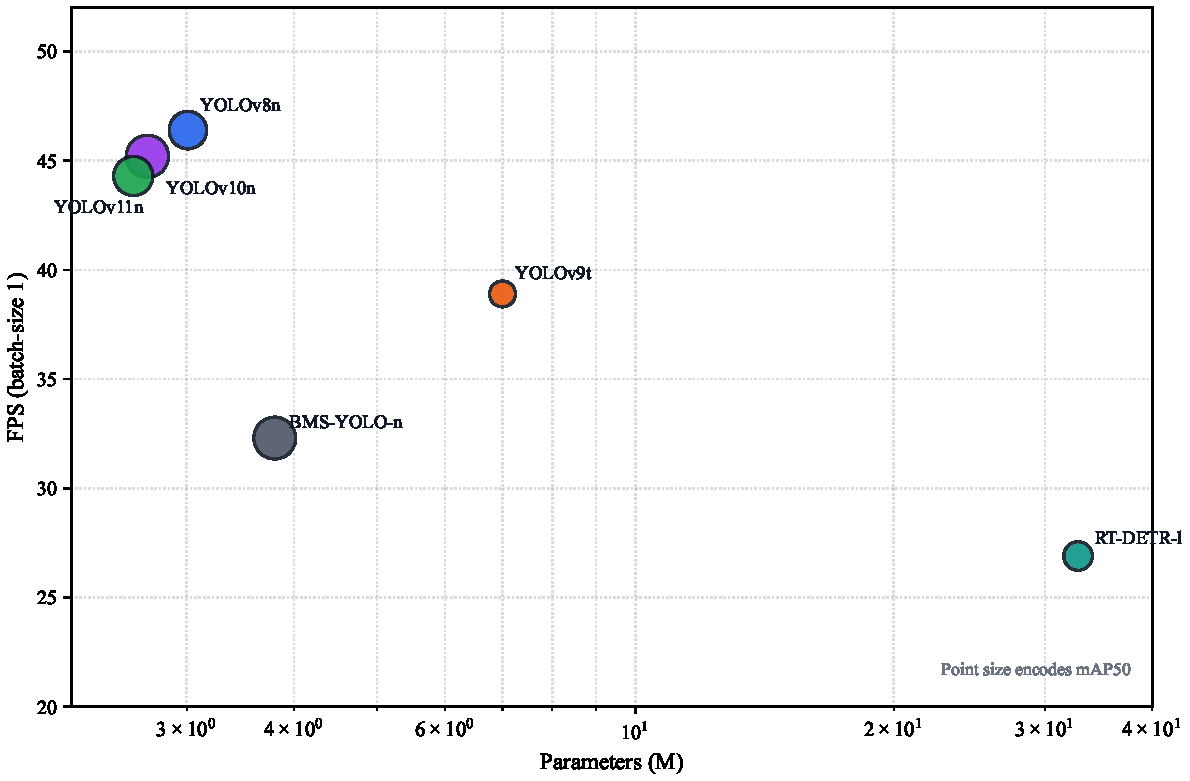
\includegraphics[width=\linewidth]{fig6_fps_params.pdf}
\caption{FPS vs.\ Parameters scatter plot illustrating the accuracy-efficiency trade-off of lightweight models. Each point represents a model; size encodes mAP50. BMS-YOLO-n achieves the best balance, delivering 79.3\% mAP50 with only 3.8M parameters.}
\label{fig:fps_params}
\end{figure}

\subsection{Ablation Studies}

\subsubsection{Architecture and Loss Co-design}

We first evaluate the individual contribution of each proposed architectural component by removing one module at a time from the complete BMS architecture trained with WIoU and Morphology Loss ($\lambda = 0.02$ for 300 epochs). Table~\ref{tab:component_removal} presents the results.

\begin{table*}[htbp]
\caption{Component Removal Ablation (BMS + WIoU + MorphLoss, 300 Epochs)}
\label{tab:component_removal}
\centering
\setlength{\tabcolsep}{3.5pt}
\begin{tabular}{lcccccc}
\toprule
Configuration & Params (M) & GFLOPs & mAP50 (\%) & mAP50:95 (\%) & P (\%) & R (\%) \\
\midrule
BMS + WIoU + MorphLoss (Full) & 3.8 & 9.9 & 77.4 & 50.9 & 84.4 & 69.6 \\
w/o FDDE                       & 3.75 & 9.0 & 72.1 & 45.1 & 80.0 & 67.1 \\
w/o MorphSparseMoE             & 3.75 & 8.8 & 70.4 & 44.1 & 82.5 & 65.9 \\
\bottomrule
\end{tabular}
\end{table*}

Removing either the FDDE module or the MorphSparseMoE results in a substantial performance decline (mAP50: $-5.3$ and $-7.0$ points, respectively). The larger drop from removing MorphSparseMoE indicates that morphology-adaptive expert routing is the single most impactful architectural component. The FDDE module, despite its minimal parameter increase, contributes significantly to high-frequency crack edge preservation, with a particularly large effect on mAP50:95 ($-5.8$ points), confirming its role in refining bounding box localization for elongated crack instances.

We then conduct a progressive ablation to trace the architecture---loss interaction. Starting from the YOLOv8n baseline, we first replace the backbone and neck bottleneck modules with our BMSC2f and LightSPPFCSPC (``BMS only``), then incrementally introduce WIoU and Morphology Loss ($\lambda = 0.02$). Table~\ref{tab:ablation} presents the step-by-step results.

\begin{table*}[!t]
\caption{Progressive Architecture and Loss Ablation}
\label{tab:ablation}
\centering
\setlength{\tabcolsep}{3.5pt}
\begin{tabular}{lcccccc}
\toprule
Configuration & WIoU & MorphLoss ($\lambda$) & mAP50 (\%) & mAP50:95 (\%) & P (\%) & R (\%) \\
\midrule
YOLOv8n (Baseline) & $\times$ & -- & 76.9 & 50.0 & 83.5 & 71.6 \\
BMS (Architecture) & $\times$ & 0 & 69.9 & 43.7 & 82.7 & 64.8 \\
+ WIoU             & \checkmark & 0 & 72.6 & 45.7 & 80.5 & 68.3 \\
+ MorphLoss        & \checkmark & 0.02 & 77.4 & 50.9 & 84.4 & 69.6 \\
+ Fine-tune        & \checkmark & 0.02 $\rightarrow$ 0.005 & \textbf{79.3} & \textbf{54.6} & \textbf{89.2} & \textbf{71.2} \\
\bottomrule
\end{tabular}
\end{table*}

The ablation reveals several important insights:

\begin{enumerate}
\item \textbf{Architecture replacement alone degrades performance} (69.9\% vs.\ 76.9\% mAP50). This is an expected consequence of substituting the well-tuned C2f modules of YOLOv8n with morphologically specialized modules (FDDE, MoE-gated feature routing, and LightSPPFCSPC) that encode structural priors for elongated patterns. Under the default CIoU loss, which optimizes axis-aligned box overlap without shape awareness, these morphology-aware features lack the supervisory signal needed to align with the detection objective, leading to a suboptimal optimization landscape. This observation motivates the co-design principle at the core of our work: morphological architecture and morphology-aware loss are mutually dependent.

\item \textbf{Adding WIoU recovers 2.7 points} (69.9\% $\rightarrow$ 72.6\%). WIoU's implicit aggressive strategy for sample quality awareness provides a harder-sample-focused gradient signal that partially aligns with the BMS architecture's emphasis on structurally distinctive regions, narrowing the performance gap.

\item \textbf{Introducing Morphology Loss ($\lambda = 0.02$) is the critical step}, boosting mAP50 to 77.4\% and surpassing the baseline by 0.5 points. MorphLoss explicitly regularizes predicted boxes toward the elongated aspect ratios characteristic of pavement cracks, providing the shape prior that the BMS modules were designed to exploit. The combination of architectural morphology awareness and morphological loss regularization validates our co-design hypothesis.

\item \textbf{Two-stage fine-tuning ($\lambda: 0.02 \rightarrow 0.005$) yields the best performance} (79.3\% mAP50, 54.6\% mAP50:95). The ``strong-to-weak'' schedule first imposes an aggressive morphological constraint to shape the feature representation, then relaxes it to allow WIoU to refine bounding box localization. This two-stage strategy contributes an additional 1.9 points over single-stage training with $\lambda = 0.02$.

% Vector PDF: Fig. 3 -- Ablation Study Bar Chart
\begin{figure}[t]
\centering
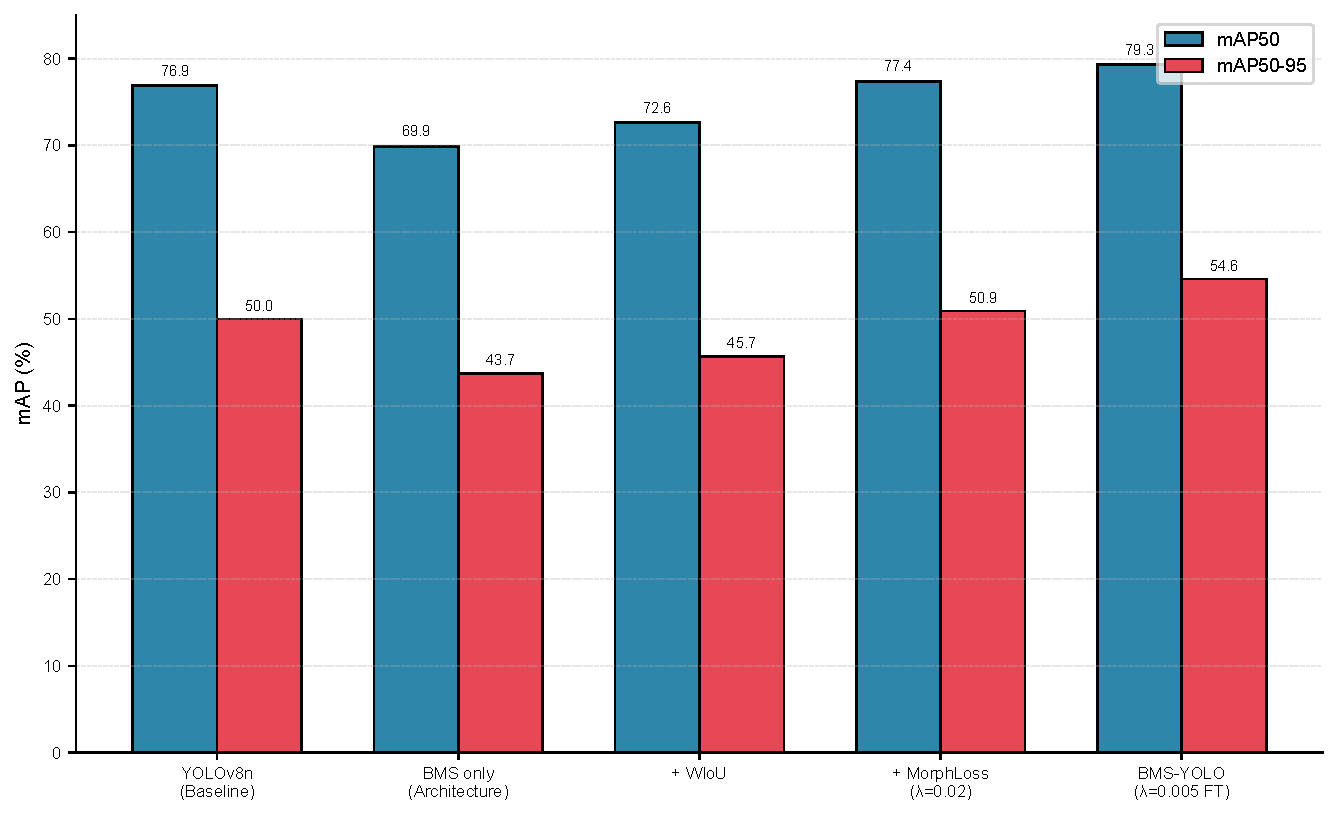
\includegraphics[width=\linewidth]{fig3_ablation.pdf}
\caption{Progressive ablation showing the contribution of each proposed component. The x-axis shows the progressive configurations: Baseline, BMS only, +WIoU, +MorphLoss ($\lambda=0.02$), and Full BMS-YOLO (two-stage $\lambda: 0.02 \rightarrow 0.005$). Grouped bars report mAP50 and mAP50:95. The architecture-only replacement degrades performance (69.9\% vs.\ 76.9\%), demonstrating that morphological modules require matching supervisory signals; performance then recovers and exceeds the baseline as WIoU and Morphology Loss are incrementally added.}
\label{fig:ablation}
\end{figure}
\end{enumerate}

\subsubsection{Hyperparameter Sensitivity of Morphology Loss Weight}

To investigate the influence of the morphology loss weight $\lambda$, we train the complete BMS-YOLO architecture with five different $\lambda$ configurations. Table~\ref{tab:lambda} reports the results.

\begin{table}[!t]
\caption{Sensitivity Analysis of Morphology Loss Weight $\lambda$}
\label{tab:lambda}
\centering
\setlength{\tabcolsep}{4pt}
\begin{tabular}{clc}
\toprule
$\lambda$ & Training Scheme & mAP50 (\%) \\
\midrule
0.000 & Scratch & 69.9 \\
0.005 & Scratch & 70.5 \\
0.010 & Scratch & 73.2 \\
0.020 & Scratch & 77.4 \\
0.020 $\rightarrow$ 0.005 & \textbf{Pre-train + Fine-tune} & \textbf{79.3} \\
\bottomrule
\end{tabular}
\end{table}

The single-stage (from-scratch) results exhibit a monotonic increase in mAP50 with $\lambda$, indicating that stronger morphological regularization consistently benefits crack detection up to $\lambda = 0.02$. Notably, small values ($\lambda \leq 0.005$) yield marginal improvement over the architecture-only baseline, confirming that a sufficiently strong shape prior is necessary to steer the BMS modules toward meaningful morphological representations. The two-stage fine-tuning scheme ($\lambda = 0.02 \rightarrow 0.005$) achieves the highest mAP50 (79.3\%), substantially outperforming the best single-stage result (77.4\% at $\lambda = 0.02$) by 1.9 points. This validates the rationale behind the ``strong-to-weak'' strategy: an aggressive initial constraint efficiently shapes the feature space, while the subsequent relaxation prevents over-regularization and permits WIoU to refine localization precision.

% Vector PDF: Fig. 4 -- Lambda Sensitivity Line Chart
\begin{figure}[t]
\centering
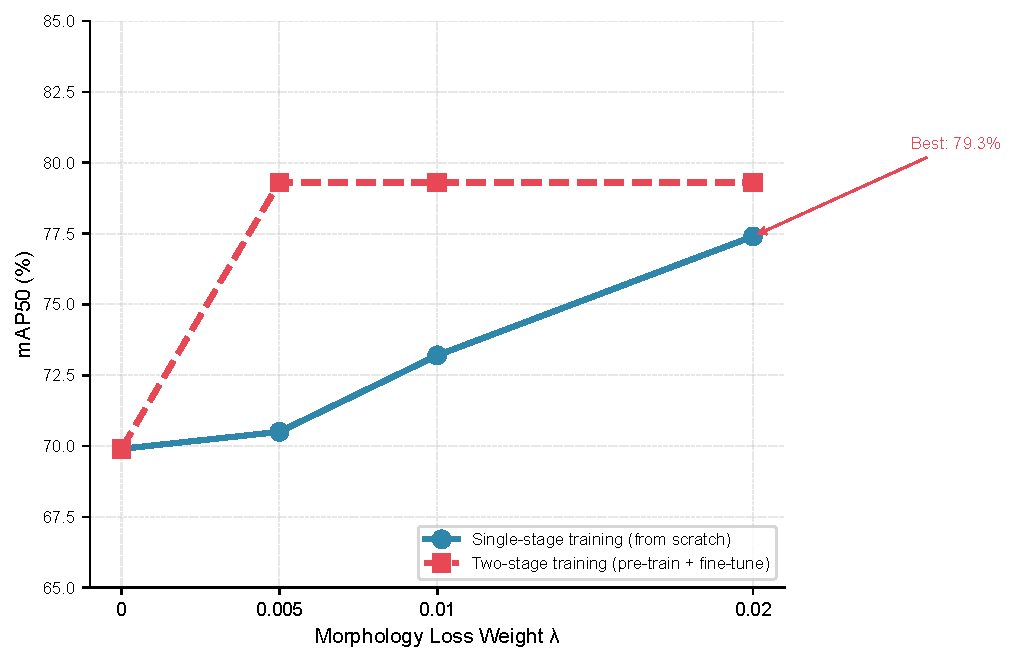
\includegraphics[width=\linewidth]{fig4_lambda_sensitivity.pdf}
\caption{Sensitivity of mAP50 to the morphology loss weight $\lambda$. The x-axis shows five configurations: $\lambda=0$, $0.005$, $0.01$, $0.02$ (all single-stage from-scratch), and $0.02 \rightarrow 0.005$ (two-stage fine-tuning). The monotonic increase with stronger $\lambda$ confirms that morphological regularization benefits crack detection, while the two-stage strategy achieves the highest performance.}
\label{fig:lambda_sensitivity}
\end{figure}

\subsubsection{Post-processing: Topology-guided Box Fusion}

Crack instances in UAV imagery often manifest as elongated, discontinuous structures that standard Non-Maximum Suppression (NMS) fragments into multiple detections. To address this, we introduce a topology-guided box fusion strategy based on a Union-Find algorithm, which merges spatially adjacent, same-class detections whose orientations are consistent with linear crack patterns.

\begin{table*}[!t]
\caption{Effect of Topology-guided Box Fusion (Post-processing Ablation)}
\label{tab:topology}
\centering
\setlength{\tabcolsep}{6pt}
\begin{tabular}{lcccc}
\toprule
Post-processing & mAP50 (\%) & mAP50:95 (\%) & P (\%) & R (\%) \\
\midrule
Standard NMS (w/o fusion) & 77.4 & 50.9 & 84.4 & 69.6 \\
+ Topology Fusion & 77.2 & 50.8 & 81.6 & \textbf{71.5} \\
\bottomrule
\end{tabular}
\end{table*}

The application of topology fusion yields a near-identical mAP50 (77.4 vs.\ 77.2) while increasing Recall by 1.9 points (69.6\% $\rightarrow$ 71.5\%), at the cost of a 2.8-point Precision drop. This trade-off reflects the nature of the COCO evaluation protocol when applied to elongated crack instances: merging multiple fragmented boxes along a single crack reduces false negatives (improving Recall) but can produce merged boxes whose IoU with any individual ground-truth annotation decreases (lowering Precision). For pavement distress inspection, where minimizing missed detections is operationally critical, the Recall gain is more practically meaningful than the marginal mAP change. The topology fusion experiment is evaluated on the 300-epoch MorphLoss checkpoint. As a model-agnostic post-processing step, it can be applied to the output of any detector; however, the actual Recall---Precision trade-off will depend on the number, position, and confidence distribution of the input detections, which vary across training checkpoints. We acknowledge that the fusion was not re-evaluated on the final 400-epoch model, and leave this for future work. Moreover, topology fusion serves as a lightweight post-processing step that does not affect training-time inference speed, making it a low-cost enhancement for real-world deployment.

\subsection{Model Complexity and Inference Efficiency}
\label{sec:complexity}

A practical detection model for UAV-based infrastructure inspection must balance accuracy against computational budget. Lightweight feature fusion designs such as Slim-Neck~\cite{ye2025yolov8nsbp} and YOLOv8n-SBP~\cite{ye2025yolov8nsbp} demonstrate that cross-stage partial networks can achieve real-time inference on edge devices. Models like GSB-YOLO~\cite{li2024lcsnet} employ ghost convolution for multi-scale fusion, while YOLO-DS~\cite{wang2026directionaware} introduces dual-statistic synergy modules for heterogeneous targets. For low-altitude UAV inspection, low-parameter detectors such as YOLO-SCX~\cite{liu2025freqyolo} further compress model size. Table~\ref{tab:complexity} compares BMS-YOLO-n with representative lightweight detectors across four efficiency dimensions.

\begin{table}[!t]
\caption{Model Complexity and Efficiency Comparison}
\label{tab:complexity}
\centering
\setlength{\tabcolsep}{4pt}
\begin{tabular}{lcccc}
\toprule
Model & Params (M) & GFLOPs & FPS & Model Size (MB) \\
\midrule
YOLOv8n  & 3.01 & 8.1 & 46.4 & $\sim$6.0 \\
YOLOv10n & $\sim$2.7 & $\sim$8 & 45.2 & $\sim$5.4 \\
BMS-YOLO-n & 3.8 & 9.9 & 32.3 & $\sim$8.1 \\
\bottomrule
\end{tabular}
\end{table}

BMS-YOLO-n introduces a modest increase in parameters (+26\% over YOLOv8n) and FLOPs (+22\%). This results in an inference speed of 32.3 FPS on an RTX 5090 GPU. Although this represents a reduction of 14.1 FPS relative to YOLOv8n, the model remains well above the 30 FPS threshold commonly regarded as the boundary for near-real-time operation. The speed reduction stems primarily from the FDDE module and MoE-gated routing in BMSC2f. These components introduce additional convolutional paths and conditional computation. The cumulative effect of these modules across all backbone and neck stages accounts for the overall increase from 3.01M to 3.8M parameters and from 8.1 to 9.9 GFLOPs.

For the target deployment scenario---UAV-based pavement inspection---the operational paradigm is predominantly offline. Images are captured during flight and processed post-mission, where detection quality takes precedence over streaming throughput. The 5,184$\times$3,888 original images are resized to 640$\times$640 via letterbox (aspect-ratio-preserving scaling with padding) for inference. At 32.3 FPS, processing a single full-resolution image requires approximately 31~ms. This makes BMS-YOLO-n suitable for batch processing of entire flight missions without operational bottleneck.

A practical consideration of the whole-image letterbox approach is that linear dimensions are reduced by approximately 8$\times$, which may attenuate fine crack details. Alternative strategies such as tiling with overlap could preserve local resolution but increase inference latency by 4$\times$ or more, and introduce boundary artifacts at tile seams. We adopted whole-image letterbox as a reasonable compromise for the offline processing scenario, acknowledging that tiling may be warranted when detecting sub-pixel-width cracks at higher flight altitudes.

\subsection{Category-wise Performance Analysis}

To understand how BMS-YOLO performs across different distress types, we report per-category mAP50 in Table~\ref{tab:category}.

\begin{table}[!t]
\caption{Per-category mAP50 Comparison: YOLOv8n vs.\ BMS-YOLO-n}
\label{tab:category}
\centering
\setlength{\tabcolsep}{4pt}
\begin{tabular}{lccc}
\toprule
Category & YOLOv8n (Baseline) & BMS-YOLO-n (Ours) & $\Delta$ (p.p.) \\
\midrule
Alligator crack    & 85.3 & \textbf{87.6} & +2.3 \\
Longitudinal crack & 73.1 & \textbf{76.1} & +3.0 \\
Oblique crack      & 66.1 & \textbf{67.5} & +1.4 \\
Pothole            & 71.9 & 71.0 & --0.9 \\
Repair             & 88.2 & \textbf{93.2} & +5.0 \\
Transverse crack   & 75.7 & \textbf{80.3} & +4.6 \\
\midrule
Overall mAP50 & 76.9 & \textbf{79.3} & +2.4 \\
\bottomrule
\end{tabular}
\end{table}

BMS-YOLO-n achieves improvements on five of six categories. The most substantial gains appear in Repair (+5.0 points) and Transverse Crack (+4.6 points). We observe that the FDDE module may contribute to the Repair improvement by capturing irregular boundaries through its frequency-direction decoupling. For Transverse Crack---a thin, horizontal linear pattern---the Morphology Loss may help guide the network toward elongated box predictions, addressing the limitation of the default CIoU loss, which provides only relative aspect ratio supervision without constraining boxes toward elongated geometries. These observations are consistent with our co-design hypothesis, though we acknowledge that without category-level ablation, we cannot definitively isolate each component's per-class contribution.

The three crack sub-categories (Alligator, Longitudinal, and Oblique) show consistent but more modest improvements (+1.4 to +3.0 points), reflecting the inherent difficulty of distinguishing crack textures from road markings and natural wear patterns in high-resolution UAV imagery.

The slight decline on Pothole (--0.9 points) may reflect the model's inherent bias toward elongated patterns in extreme long-tail scenarios. The test set contains only 17 Pothole instances (1.4\% of all test annotations), placing this category in a regime where single-sample variation has a disproportionate effect on mAP. The overall accuracy gain of 2.4 points suggests that the morphological design benefits linear distress types without substantially harming compact defect detection.

% Vector PDF: Fig. 5 -- Per-Category mAP50 Comparison Bar Chart
\begin{figure}[t]
\centering
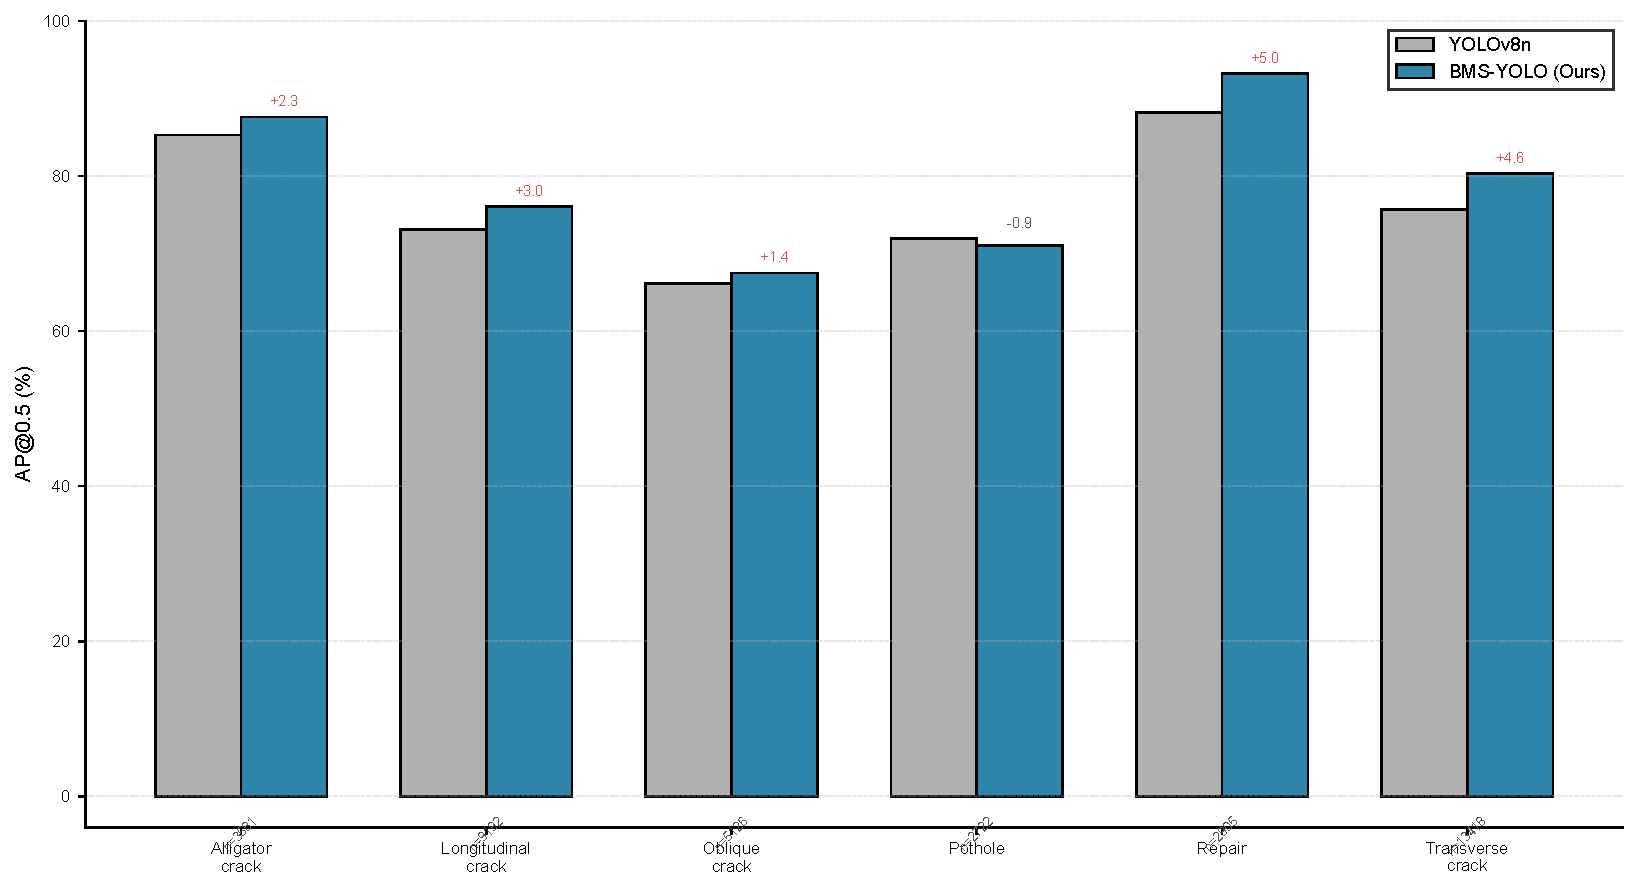
\includegraphics[width=\linewidth]{fig5_category_comparison.pdf}
\caption{Per-category mAP50 comparison between YOLOv8n and BMS-YOLO-n across the six distress types. Grouped bars show that BMS-YOLO-n improves all linear defect categories (Transverse +4.6, Longitudinal +3.0, Alligator +2.3, Oblique +1.4) and achieves the largest gain on Repair (+5.0), while Pothole experiences a marginal decline (--0.9) attributable to the extreme class imbalance (only 17 test instances).}
\label{fig:category_comparison}
\end{figure}

\subsection{Qualitative Results}

To complement the quantitative analysis, we present visual comparisons between YOLOv8n (baseline) and BMS-YOLO-n on three representative UAV-PDD2023 test samples, each highlighting a distinct failure mode of the baseline.

% Vector PDF figures (qualitative_fig_1/2/3) replace original JPG images.

\begin{figure}[t]
\centering
\includegraphics[width=\linewidth]{qualitative_fig_1.pdf}
\caption{Faint transverse crack near double-yellow lane markings. Left column: original cropped image. Middle column: YOLOv8n detects ``Transverse crack'' at low confidence (0.39) with a loosely fitted box. Right column: BMS-YOLO-n raises confidence to 0.47 and produces a tighter bounding box that better follows the crack geometry, consistent with the expected effect of Morphology Loss in resolving aspect-ratio ambiguity.}
\label{fig:qual1}
\end{figure}

\begin{figure}[t]
\centering
\includegraphics[width=\linewidth]{qualitative_fig_2.pdf}
\caption{Dense multi-class distress scene. Left column: original cropped image. Middle column: YOLOv8n fragments the same crack into multiple overlapping boxes with confidences ranging from 0.61 to 0.80, and assigns Repair a confidence of only 0.78. Right column: BMS-YOLO-n yields a more coherent detection set with higher confidences (Repair: 0.89; Oblique crack: 0.83) and fewer redundant boxes, consistent with the role of topology-guided fusion.}
\label{fig:qual2}
\end{figure}

\begin{figure}[t]
\centering
\includegraphics[width=\linewidth]{qualitative_fig_3.pdf}
\caption{Co-occurring pothole and transverse crack. Left column: original cropped image. Middle column: YOLOv8n detects Pothole at 0.75--0.76 confidence. Right column: BMS-YOLO-n increases Pothole confidence to 0.88--0.89 and Transverse Crack to 0.87--0.88, suggesting that WIoU may help elevate the quality of rare-class predictions despite the extreme class imbalance.}
\label{fig:qual3}
\end{figure}

As shown in Fig.~\ref{fig:qual1}, a faint transverse crack crosses double-yellow lane markings. YOLOv8n assigns a low confidence score (Transverse Crack: 0.39) and produces a bounding box with excessive vertical padding. BMS-YOLO-n raises the confidence to 0.47 and tightens the box to better follow the crack geometry, which is consistent with the expected effect of Morphology Loss in resolving aspect-ratio ambiguity. In Fig.~\ref{fig:qual2}, a dense multi-class scene contains Repair, Oblique Crack, and Longitudinal Crack regions. YOLOv8n fragments the same crack into three to four separate boxes with confidences ranging from 0.61 to 0.80. BMS-YOLO-n, by contrast, produces a more coherent set of detections with higher confidences (Repair: 0.89 vs.\ 0.78; Oblique Crack: 0.83 vs.\ 0.80), consistent with the role of topology-guided fusion in merging spatially adjacent detections along linear crack trajectories. Finally, Fig.~\ref{fig:qual3} shows a co-occurring pothole and transverse crack scenario. Despite the extreme class imbalance that places Pothole in the long-tail regime, BMS-YOLO-n increases Pothole detection confidence from 0.75--0.76 to 0.88--0.89, suggesting that the WIoU loss may help elevate the quality of rare-class predictions.

\subsection{Discussion}

The experimental results collectively validate the co-design philosophy underlying BMS-YOLO. The component removal ablation (Table~\ref{tab:component_removal}) demonstrates that each proposed architectural module contributes individually. Removing MorphSparseMoE causes the largest drop (mAP50: $-7.0$ points). This confirms morphology-adaptive expert routing as the most impactful component. FDDE removal still reduces mAP50 by 5.3 points, validating the importance of frequency---direction decoupling for crack edge preservation. The progressive ablation (Table~\ref{tab:ablation}) further demonstrates that the architectural modifications and loss functions are mutually reinforcing. The BMS modules provide morphology-sensitive feature representations. WIoU and MorphLoss supply the complementary gradient signals needed to exploit them. The hyperparameter analysis (Table~\ref{tab:lambda}) identifies the ``strong-to-weak'' two-stage training as the optimal strategy for leveraging morphological priors.

A limitation worth noting is the inference speed reduction relative to the YOLOv8n baseline (Section~\ref{sec:complexity}). While the 32.3 FPS achieved by BMS-YOLO-n remains suitable for offline UAV inspection pipelines, future work could explore architecture distillation or neural architecture search to further compress the FDDE and MoE components without sacrificing the morphological advantage. Additionally, the mild Recall gain from topology fusion (Table~\ref{tab:topology}) comes at the cost of Precision; integrating topology awareness directly into the training objective, rather than as a post-processing step, represents a promising direction for end-to-end optimization.

Another limitation concerns the MorphSparseMoE expert design. The horizontal and vertical expert kernels are defined relative to the image coordinate system, whereas the semantic categories ``Transverse'' and ``Longitudinal'' are defined relative to the road axis. Since UAV imagery can be captured at arbitrary headings, the alignment between expert orientation and distress semantics is not guaranteed. A rotation-aware expert design or road-axis normalization would address this mismatch, and we leave it for future work. Furthermore, the per-category performance analysis (Table~\ref{tab:category}) is based on a single random seed, and we do not report uncertainty estimates. Category-level ablation to isolate each component's per-class contribution is also left for future investigation.

\section{Conclusion}
\label{sec:concl}

This paper presented BMS-YOLO, a lightweight detection framework for pavement distress detection that addresses three fundamental limitations of standard YOLO architectures: high-frequency detail loss, insufficient morphological adaptability, and loss function misalignment with crack geometry. The central contribution of this work is the \textit{architecture---loss co-design philosophy}: morphology-aware architectural modules (FDDE, MorphSparseMoE) provide structural inductive biases tailored to elongated crack patterns, while morphology-sensitive supervisory signals (WIoU and morphology consistency loss) supply the complementary gradient needed to activate and refine these biases. Neither component alone is sufficient; the progressive ablation study confirms that architectural replacement degrades performance without the matching loss, while the full co-design achieves consistent gains across all evaluation metrics.

BMS-YOLO achieves 79.3\% mAP50 and 54.6\% mAP50:95 on UAV-PDD2023, outperforming YOLOv8n by 2.4 and 4.6 points respectively, while maintaining 32.3 FPS on a desktop GPU. The topology-guided box fusion post-processing strategy further increases recall by 1.9 points for fragmented crack detection. These results demonstrate that the model offers both the accuracy and efficiency required for UAV-based pavement inspection pipelines.

\textbf{Limitations:} Despite the overall performance gains, several limitations remain. First, the model still struggles with extremely low-contrast cracks where the intensity difference between the defect and the background is minimal. Second, dense mesh-like crack networks present a challenge for current topology fusion, as the Union-Find algorithm may over-merge intersecting crack segments. Third, the inference speed of BMS-YOLO is reduced by approximately 30\% compared with YOLOv8n, primarily due to the additional computational cost of FDDE and MorphSparseMoE modules. Fourth, the slight decline on Pothole detection ($-$0.9 points) may reflect the model's inherent bias toward elongated patterns in extreme long-tail scenarios, though we cannot rule out stochastic effects. Fifth, the MorphSparseMoE horizontal and vertical experts are defined relative to the image coordinate system, whereas the semantic categories ``Transverse'' and ``Longitudinal'' are defined relative to the road axis; this mismatch may limit expert effectiveness under varying UAV flight headings. Sixth, all reported results are based on a single random seed, and we do not provide uncertainty estimates; multi-seed experiments with confidence intervals are needed for more robust conclusions.

\textbf{Future Work:} We plan to address these limitations through a phased research roadmap. \textit{Short-term} efforts will focus on model compression: INT8 quantization and structured pruning of FDDE and MoE components to reduce the parameter count and improve edge deployment on UAV-borne hardware (e.g., NVIDIA Jetson series). \textit{Mid-term} work will explore illumination normalization preprocessing or Retinex-based low-frequency compensation to enhance low-contrast crack responses, as well as graph neural networks for improved topological modeling of dense mesh-like crack networks. \textit{Long-term} directions include investigating semi-supervised and weakly supervised learning paradigms to reduce reliance on large-scale accurate bounding box annotations, and extending the co-design framework to other morphologically diverse detection domains such as railway defect inspection and bridge structural health monitoring.

\bibliographystyle{IEEEtran}
\bibliography{references}

\begin{IEEEbiography}[{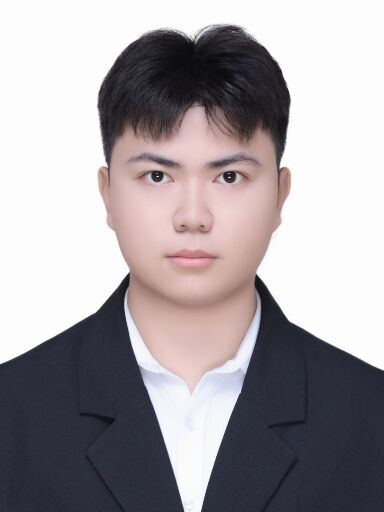
\includegraphics[width=1in,height=1.25in,clip,keepaspectratio]{author_qi_liu.jpg}}]{Qi Liu} received the B.S. degree from Yangtze Normal University, Chongqing, China. He is currently pursuing research in intelligent infrastructure inspection and deep learning-based pavement distress detection at the College of Big Data and Intelligent Engineering, Yangtze Normal University. His research interests include computer vision for civil infrastructure, lightweight object detection models, UAV-based remote sensing, and morphology-aware neural network design.

\end{IEEEbiography}

\EOD
\end{document}
